\documentclass[12pt,a4paper]{article}

%\pdfoutput=1

\usepackage[utf8]{inputenc}
\usepackage[T1]{fontenc}
\usepackage[english]{babel}
\usepackage{amsmath}
\usepackage{lmodern}
\usepackage{units}
\usepackage{siunitx}
\usepackage{icomma}
\usepackage{graphicx}
\usepackage{caption}
\usepackage{subcaption}
\usepackage{color}
\newcommand{\N}{\ensuremath{\mathbbm{N}}}
\newcommand{\Z}{\ensuremath{\mathbbm{Z}}}
\newcommand{\Q}{\ensuremath{\mathbbm{Q}}}
\newcommand{\R}{\ensuremath{\mathbbm{R}}}
\newcommand{\C}{\ensuremath{\mathbbm{C}}}
\newcommand{\rd}{\ensuremath{\mathrm{d}}}
\newcommand{\id}{\ensuremath{\,\rd}}
\usepackage{hyperref}
%\usepackage{a4wide} % puts the page numbering further down the page.
\usepackage{pdfpages}
\usepackage{epstopdf}
\DeclareGraphicsExtensions{.eps}

\title{3D Lab Homework}
\author{Marcus Malmquist, marmalm, 941022}
\date{\today}

\begin{document}
\maketitle

\section{Task 1}\label{sec:1}
The waveguide used in this simulation was a single waveguide with the dimensions $(x=\SI{10}{\milli\metre}, y=\SI{40}{\milli\metre}, z=\SI{50}{\milli\metre})$. The wave propagated in the $z$-direction. Some of the results of the simulation can be seen in Figure~\ref{fig:task1}.

The cutoff frequency can be calculated using (\ref{eq:cutoff}). For a hollow wave guide ($\mu_r\approx 1, \epsilon_r\approx 1$) with these dimensions ($a=\SI{40}{\milli\metre}$, $b=\SI{10}{\milli\metre}$) the theoretical cutoff frequency is $\SI{7.5}{\giga\hertz}$. From Figure~\ref{fig:1_s1222} it can be seen that the simulated cutoff frequency is also $\SI{7.5}{\giga\hertz}$.
\begin{equation}
  f_{\text{cutoff},m,n}=\frac{c}{2\sqrt{\mu_r\epsilon_r}}\sqrt{\big(\frac{m}{a}\big)^2+\big(\frac{n}{b}\big)^2}
  \label{eq:cutoff}
\end{equation}

\begin{figure}
  \centering
  \begin{subfigure}[b]{0.49\textwidth}
    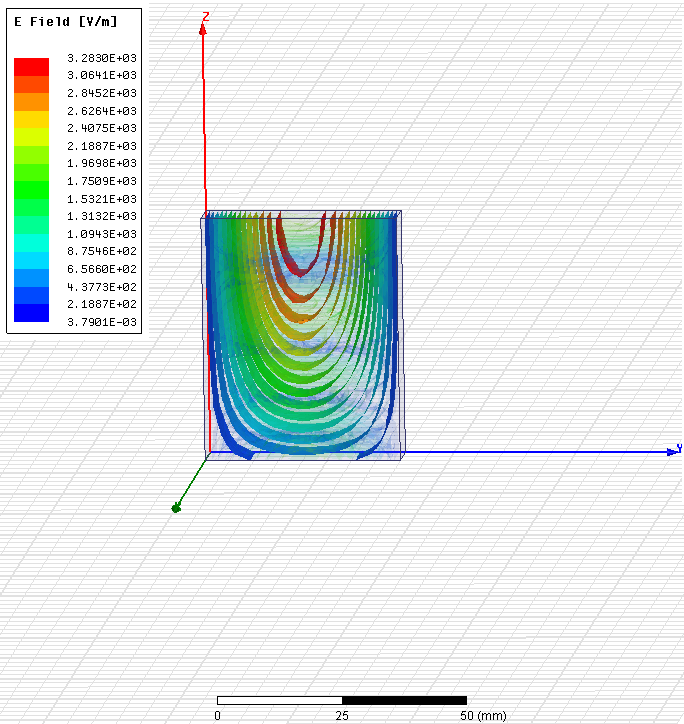
\includegraphics[width=\textwidth]{./HFSSDesign1/4ghz.png}
    \subcaption{The magnitude of the E-field at $f=\SI{4}{\giga\hertz}$.}
    \label{fig:1_4ghz}
  \end{subfigure}
  \begin{subfigure}[b]{0.49\textwidth}
    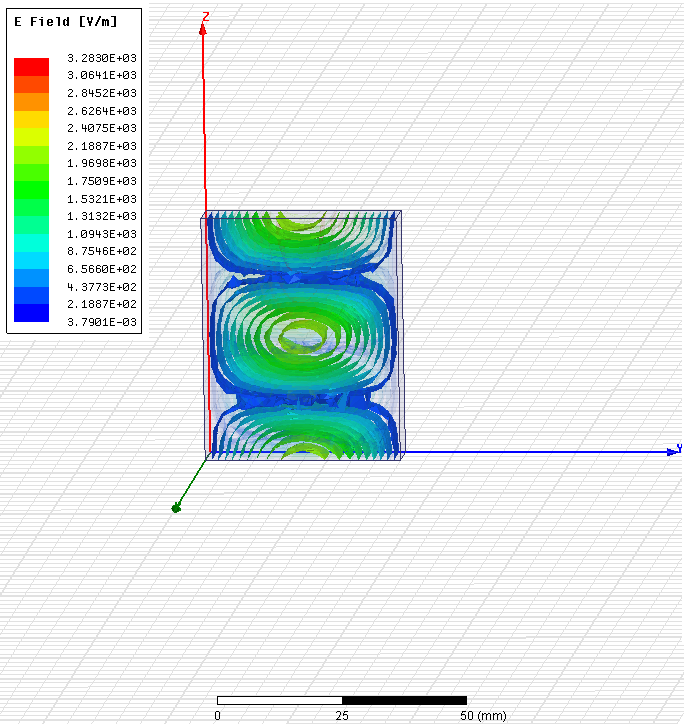
\includegraphics[width=\textwidth]{./HFSSDesign1/7ghz.png}
    \subcaption{The magnitude of the E-field at $f=\SI{7}{\giga\hertz}$.}
    \label{fig:1_7ghz}
  \end{subfigure}\\
  \begin{subfigure}[b]{0.49\textwidth}
    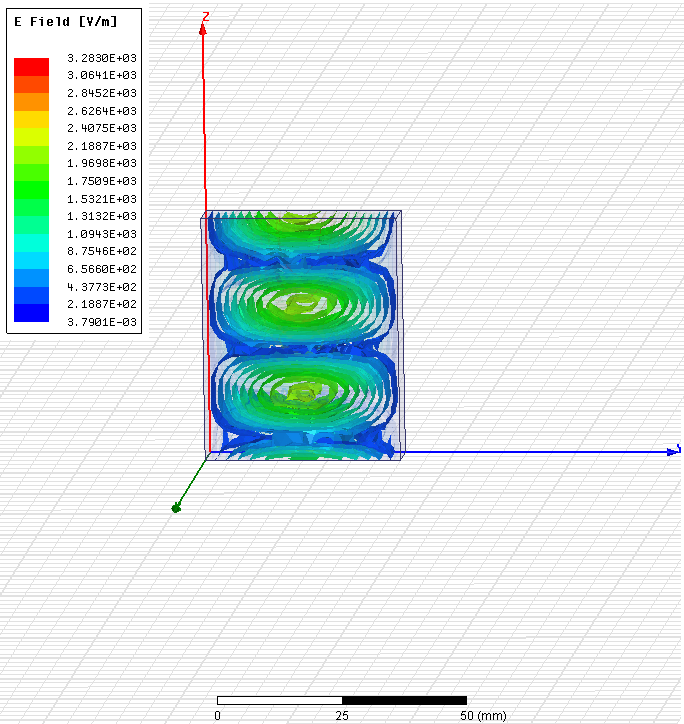
\includegraphics[width=\textwidth]{./HFSSDesign1/9ghz.png}
    \subcaption{The magnitude of the E-field at $f=\SI{9}{\giga\hertz}$.}
    \label{fig:1_9ghz}
  \end{subfigure}
  \begin{subfigure}[b]{0.49\textwidth}
    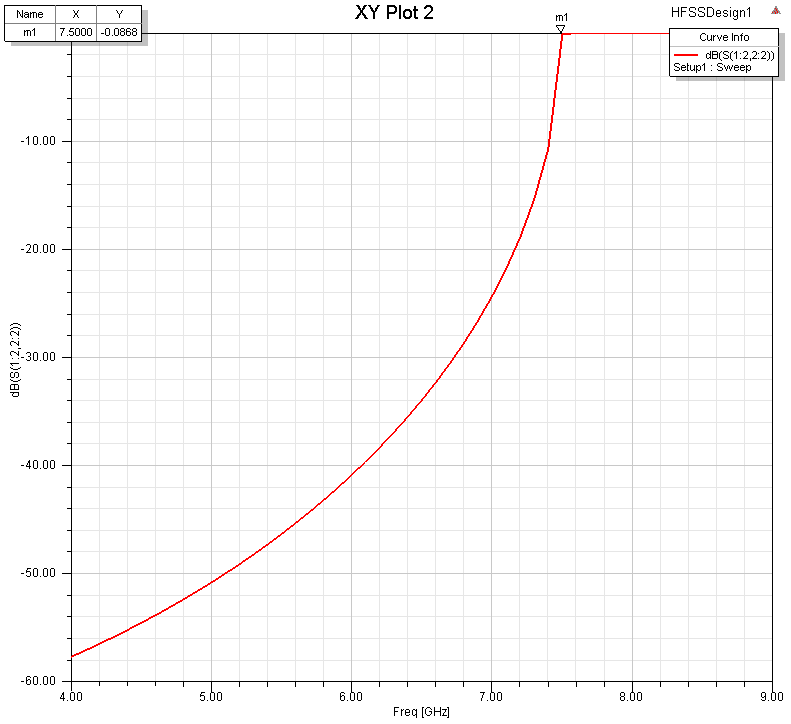
\includegraphics[width=\textwidth]{./HFSSDesign1/s1222.png}
    \subcaption{Output power of $TE_{20}$ ($S_{21}$).}
    \label{fig:1_s1222}
  \end{subfigure}
  \caption{The figure shows the magnitude of the E-field and the $S_{21}$ parameter for a waveguide with dimensions $(x=\SI{10}{\milli\metre}, y=\SI{40}{\milli\metre}, z=\SI{50}{\milli\metre})$.}
  \label{fig:task1}
\end{figure}

\section{Task 2}\label{sec:2}
In this task the wave guide was comprised of three sections. The first and the last section had the same dimensions as that which was used in Section~\ref{sec:1} $(x=\SI{10}{\milli\metre}, y=\SI{40}{\milli\metre}, z=\SI{50}{\milli\metre})$ while the middle section had varying dimensions. The $x$-dimension (``height'') was set to be the same as that of the first and last sections $(x=\SI{10}{\milli\metre})$. This design should essensially by a high-pass filter since a smaller waveguide would not allow lower frequencies to propagate through it.

By comparing $S_{21}$ for all of the different dimensions of the middle section (Figure~\ref{fig:2_1050_s1222}, Figure~\ref{fig:2_3050_s1222}, Figure~\ref{fig:2_2010_s1222}, Figure~\ref{fig:2_2030_s1222}, Figure~\ref{fig:2_2050_s1222}) it can be seen that the ``width'' of the middle section matters alot more than the ``length'' of the middle section. This seems reasonable given that the theoretical cutoff frequency depends on the width and height of the wave guide, not the length of it.

\subsection{Dimensions: y=10 mm, z=50 mm}
It can be seen in Figure~\ref{fig:task2_1050} that the cutoff frequency for this wave guide is above $\SI{9}{\giga\hertz}$ since the wave does not propagate through the middle section at this frequency.
\begin{figure}
  \centering
  \begin{subfigure}[b]{0.49\textwidth}
    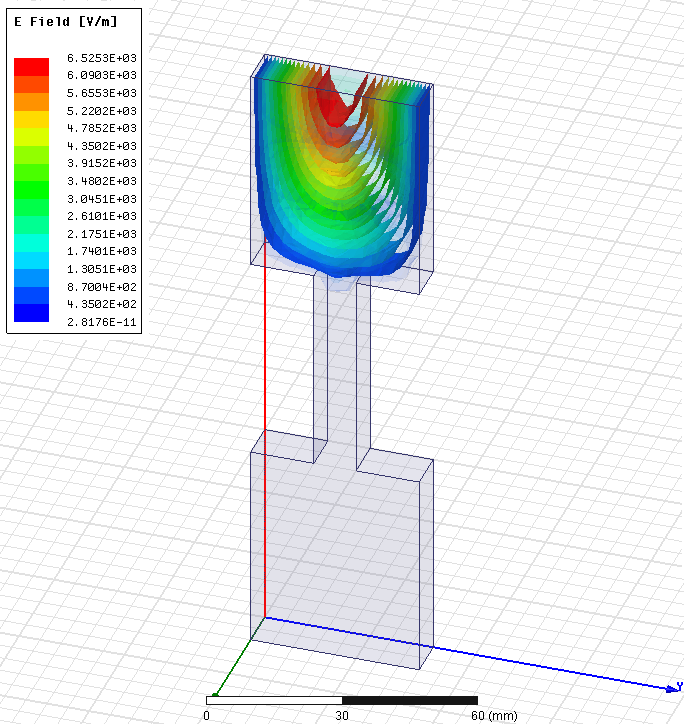
\includegraphics[width=\textwidth]{./mid_sec_10mm_wide_50mm_long/4ghz.png}
    \subcaption{The magnitude of the E-field at $f=\SI{4}{\giga\hertz}$.}
    \label{fig:2_1050_4ghz}
  \end{subfigure}
  \begin{subfigure}[b]{0.49\textwidth}
    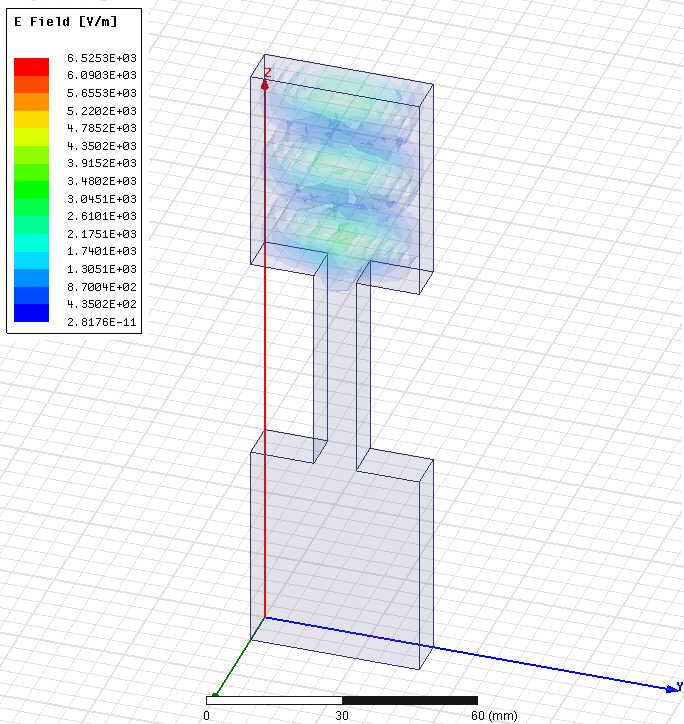
\includegraphics[width=\textwidth]{./mid_sec_10mm_wide_50mm_long/7ghz.png}
    \subcaption{The magnitude of the E-field at $f=\SI{7}{\giga\hertz}$.}
    \label{fig:2_1050_7ghz}
  \end{subfigure}\\
  \begin{subfigure}[b]{0.49\textwidth}
    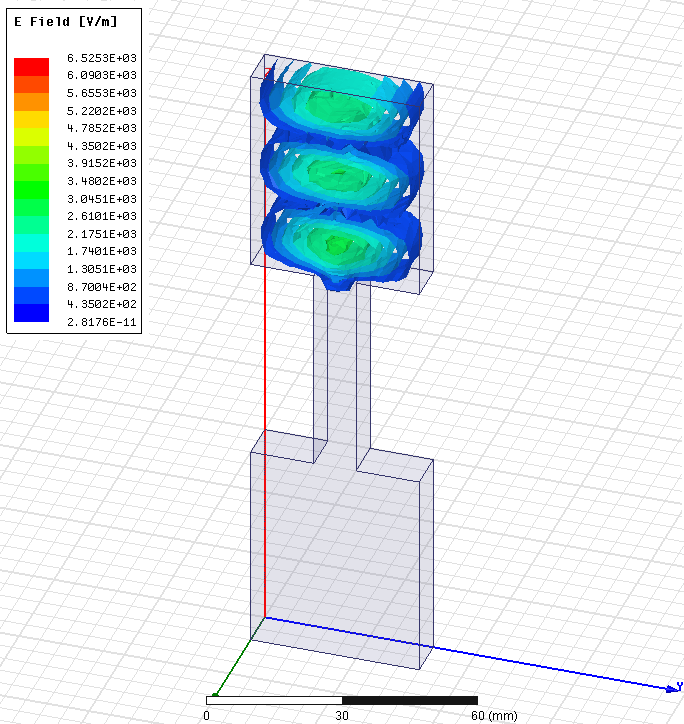
\includegraphics[width=\textwidth]{./mid_sec_10mm_wide_50mm_long/9ghz.png}
    \subcaption{The magnitude of the E-field at $f=\SI{9}{\giga\hertz}$.}
    \label{fig:2_1050_9ghz}
  \end{subfigure}
  \begin{subfigure}[b]{0.49\textwidth}
    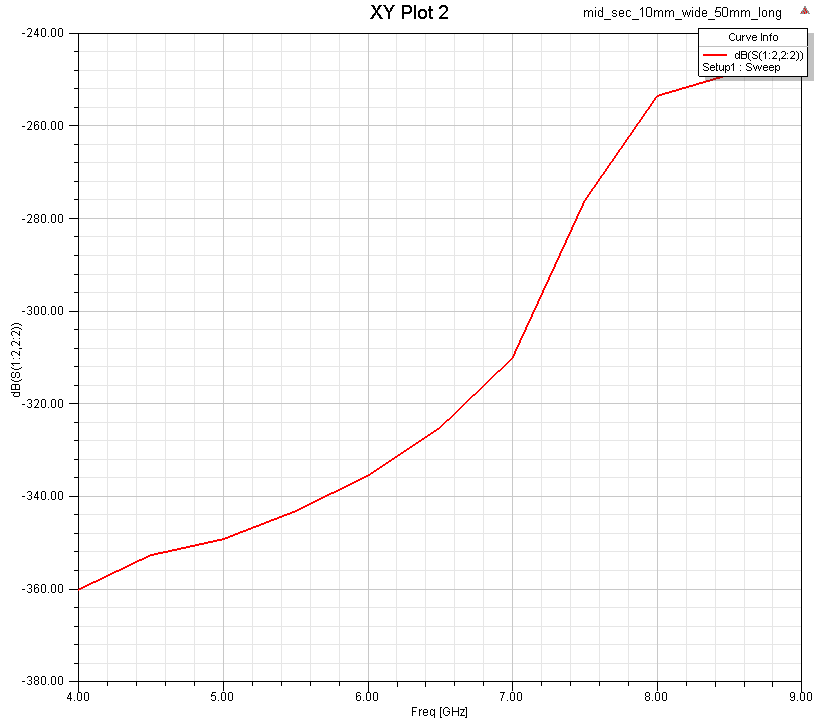
\includegraphics[width=\textwidth]{./mid_sec_10mm_wide_50mm_long/s1222.png}
    \subcaption{Output power of $TE_{20}$ ($S_{21}$).}
    \label{fig:2_1050_s1222}
  \end{subfigure}
  \caption{The figure shows the magnitude of the E-field and the $S_{21}$ parameter for a waveguide when the middle section's dimensions were $(x=\SI{10}{\milli\metre}, y=\SI{10}{\milli\metre}, z=\SI{50}{\milli\metre})$.}
  \label{fig:task2_1050}
\end{figure}

\subsection{Dimensions: y=30mm, z=50mm}
It can be seen in Figure~\ref{fig:task2_3050} that the cutoff frequency for this wave guide is just above $\SI{9}{\giga\hertz}$ although the wave manages to propagate through the middle section.
\begin{figure}
  \centering
  \begin{subfigure}[b]{0.49\textwidth}
    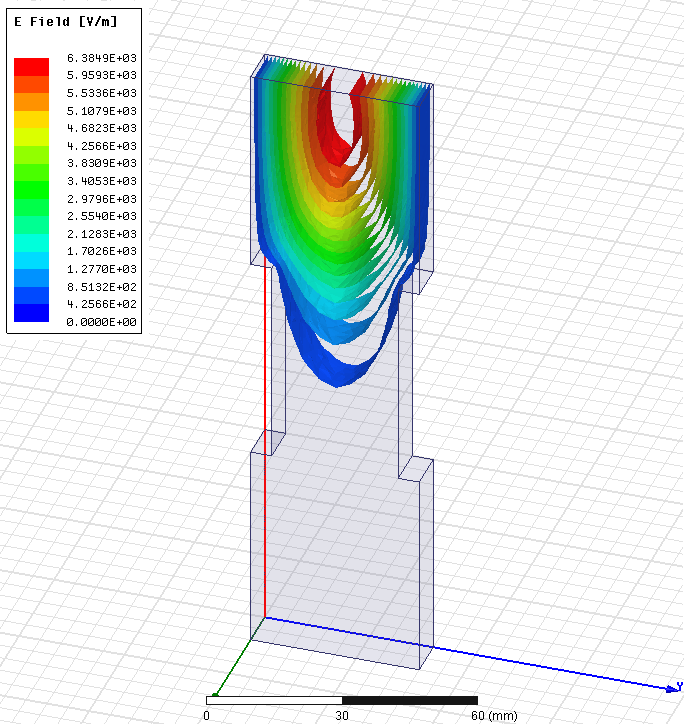
\includegraphics[width=\textwidth]{./mid_sec_30mm_wide_50mm_long/4ghz.png}
    \subcaption{The magnitude of the E-field at $f=\SI{4}{\giga\hertz}$.}
    \label{fig:2_3050_4ghz}
  \end{subfigure}
  \begin{subfigure}[b]{0.49\textwidth}
    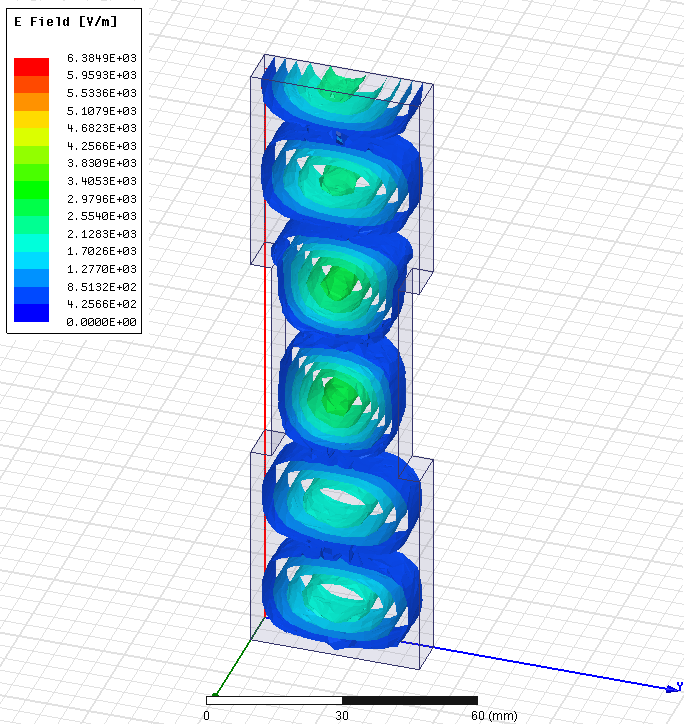
\includegraphics[width=\textwidth]{./mid_sec_30mm_wide_50mm_long/7ghz.png}
    \subcaption{The magnitude of the E-field at $f=\SI{7}{\giga\hertz}$.}
    \label{fig:2_3050_7ghz}
  \end{subfigure}\\
  \begin{subfigure}[b]{0.49\textwidth}
    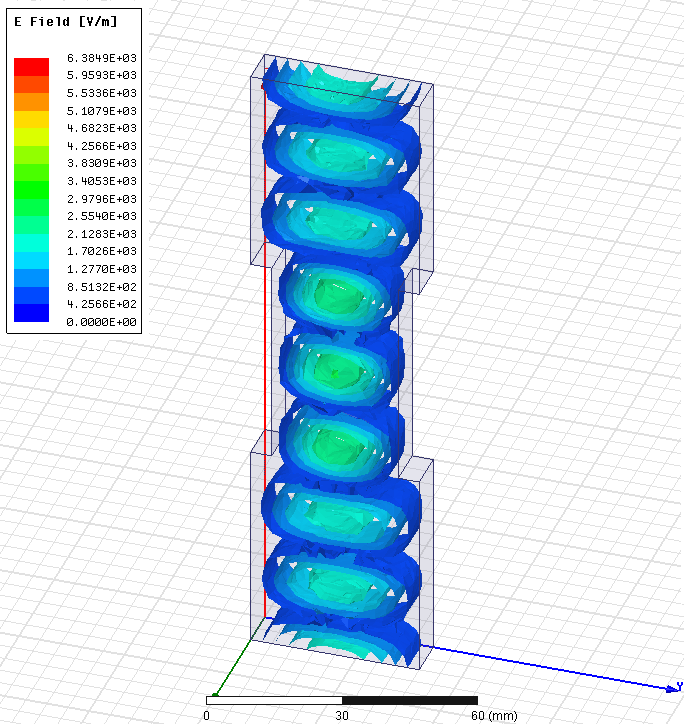
\includegraphics[width=\textwidth]{./mid_sec_30mm_wide_50mm_long/9ghz.png}
    \subcaption{The magnitude of the E-field at $f=\SI{9}{\giga\hertz}$.}
    \label{fig:2_3050_9ghz}
  \end{subfigure}
  \begin{subfigure}[b]{0.49\textwidth}
    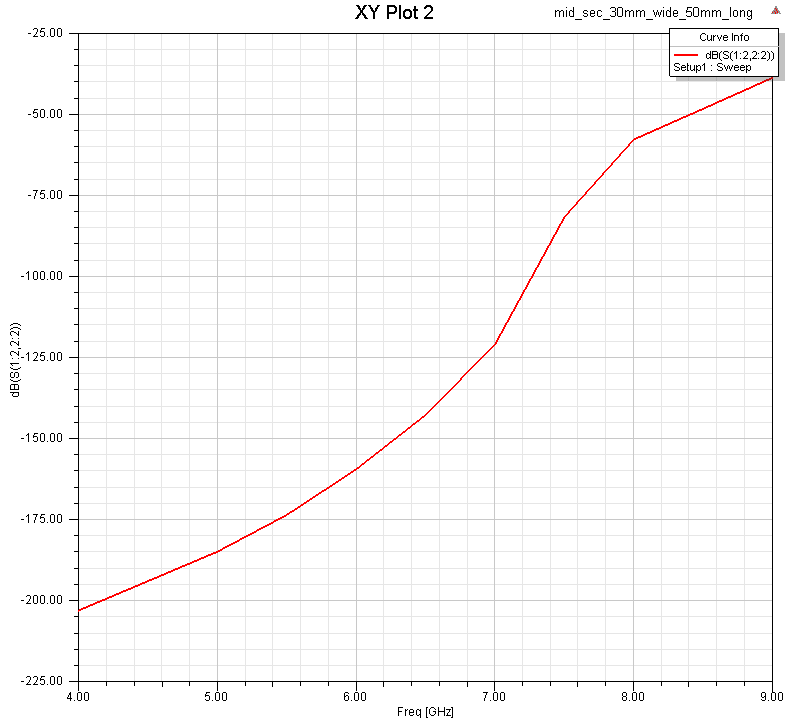
\includegraphics[width=\textwidth]{./mid_sec_30mm_wide_50mm_long/s1222.png}
    \subcaption{Output power of $TE_{20}$ ($S_{21}$).}
    \label{fig:2_3050_s1222}
  \end{subfigure}
  \caption{The figure shows the magnitude of the E-field and the $S_{21}$ parameter for a waveguide when the middle section's dimensions were $(x=\SI{10}{\milli\metre}, y=\SI{30}{\milli\metre}, z=\SI{50}{\milli\metre})$.}
  \label{fig:task2_3050}
\end{figure}

\subsection{Dimensions: y=20 mm, z=10 mm}
It can be seen in Figure~\ref{fig:task2_2010} that the cutoff frequency for this wave guide is above $\SI{9}{\giga\hertz}$ although the wave manages to propagate through the middle section.
\begin{figure}
  \centering
  \begin{subfigure}[b]{0.49\textwidth}
    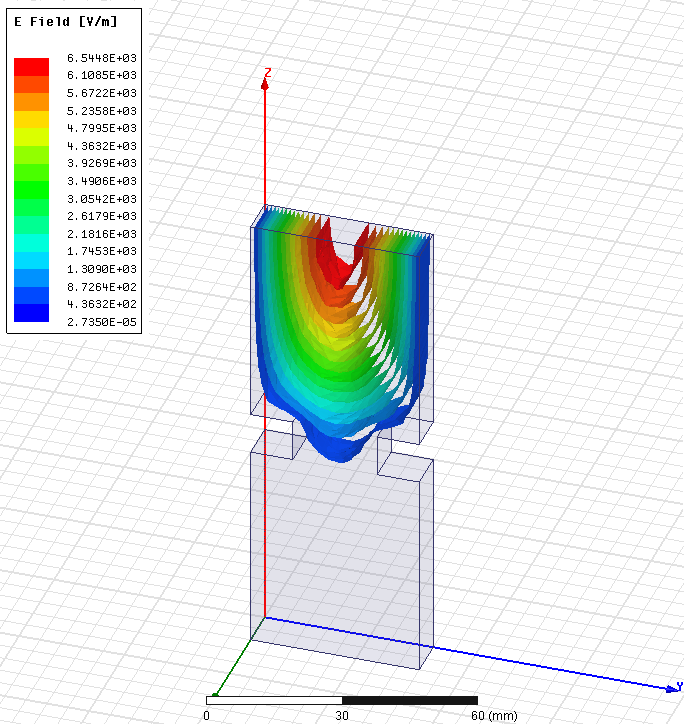
\includegraphics[width=\textwidth]{./mid_sec_20mm_wide_10mm_long/4ghz.png}
    \subcaption{The magnitude of the E-field at $f=\SI{4}{\giga\hertz}$.}
    \label{fig:2_2010_4ghz}
  \end{subfigure}
  \begin{subfigure}[b]{0.49\textwidth}
    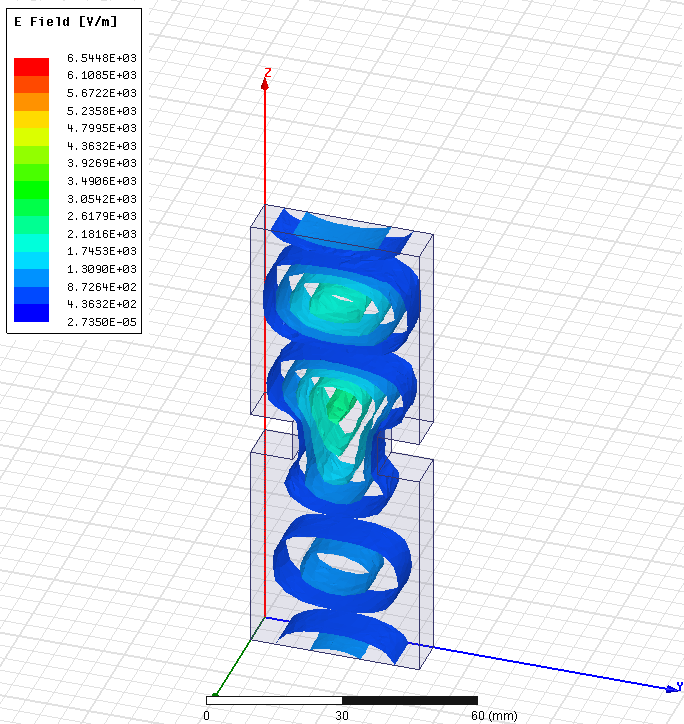
\includegraphics[width=\textwidth]{./mid_sec_20mm_wide_10mm_long/7ghz.png}
    \subcaption{The magnitude of the E-field at $f=\SI{7}{\giga\hertz}$.}
    \label{fig:2_2010_7ghz}
  \end{subfigure}\\
  \begin{subfigure}[b]{0.49\textwidth}
    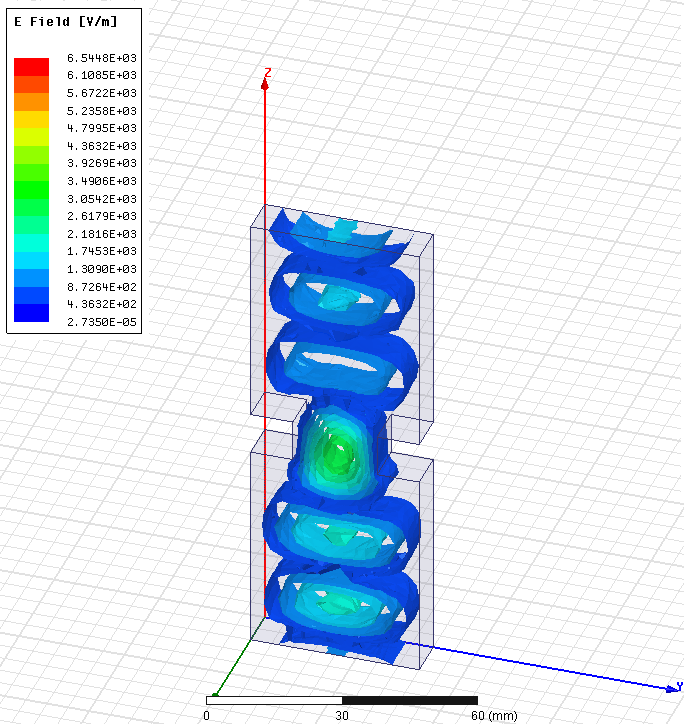
\includegraphics[width=\textwidth]{./mid_sec_20mm_wide_10mm_long/9ghz.png}
    \subcaption{The magnitude of the E-field at $f=\SI{9}{\giga\hertz}$.}
    \label{fig:2_2010_9ghz}
  \end{subfigure}
  \begin{subfigure}[b]{0.49\textwidth}
    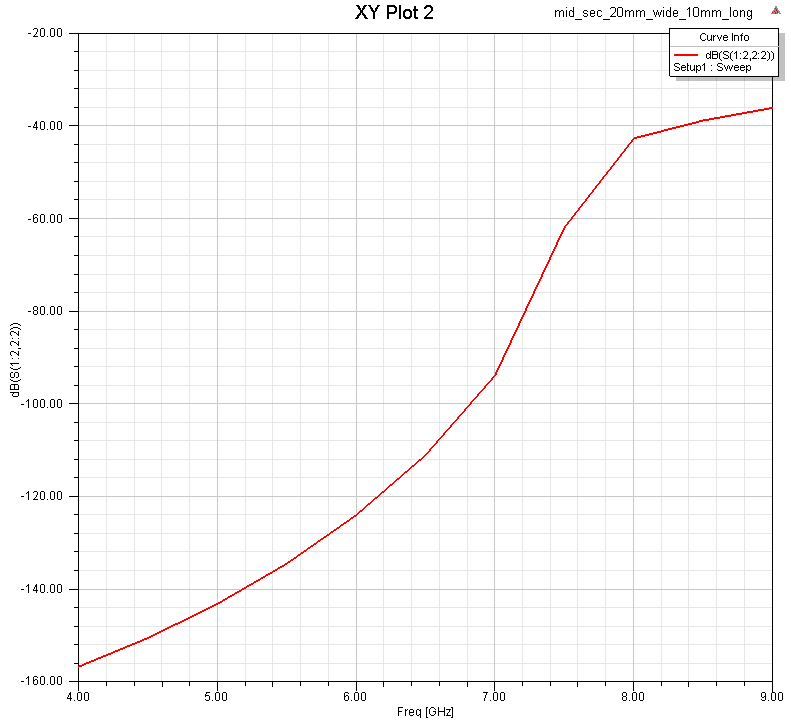
\includegraphics[width=\textwidth]{./mid_sec_20mm_wide_10mm_long/s1222.png}
    \subcaption{Output power of $TE_{20}$ ($S_{21}$).}
    \label{fig:2_2010_s1222}
  \end{subfigure}
  \caption{The figure shows the magnitude of the E-field and the $S_{21}$ parameter for a waveguide when the middle section's dimensions were $(x=\SI{10}{\milli\metre}, y=\SI{20}{\milli\metre}, z=\SI{10}{\milli\metre})$.}
  \label{fig:task2_2010}
\end{figure}

\subsection{Dimensions: y=20 mm, z=30 mm}
It can be seen in Figure~\ref{fig:task2_2030} that the cutoff frequency for this wave guide is above $\SI{9}{\giga\hertz}$ although the wave manages to propagate through the middle section.
\begin{figure}
  \centering
  \begin{subfigure}[b]{0.49\textwidth}
    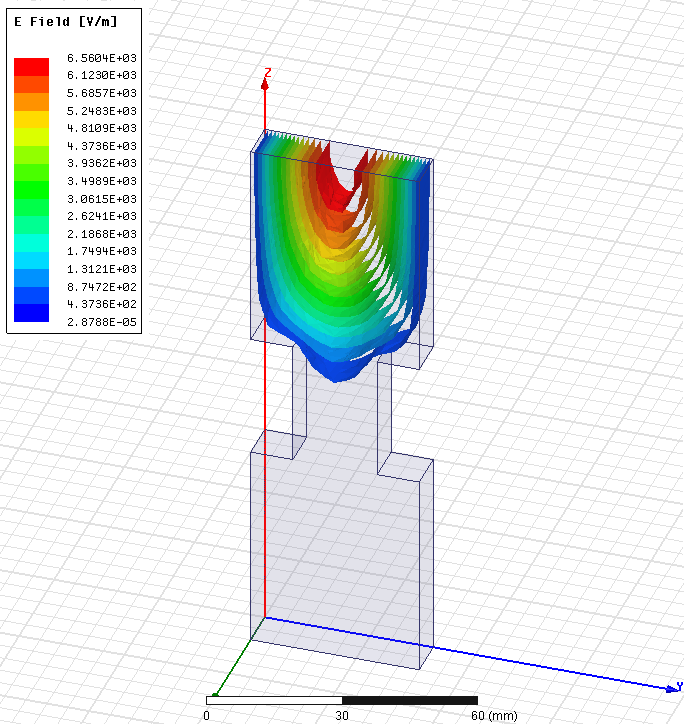
\includegraphics[width=\textwidth]{./mid_sec_20mm_wide_30mm_long/4ghz.png}
    \subcaption{The magnitude of the E-field at $f=\SI{4}{\giga\hertz}$.}
    \label{fig:2_2030_4ghz}
  \end{subfigure}
  \begin{subfigure}[b]{0.49\textwidth}
    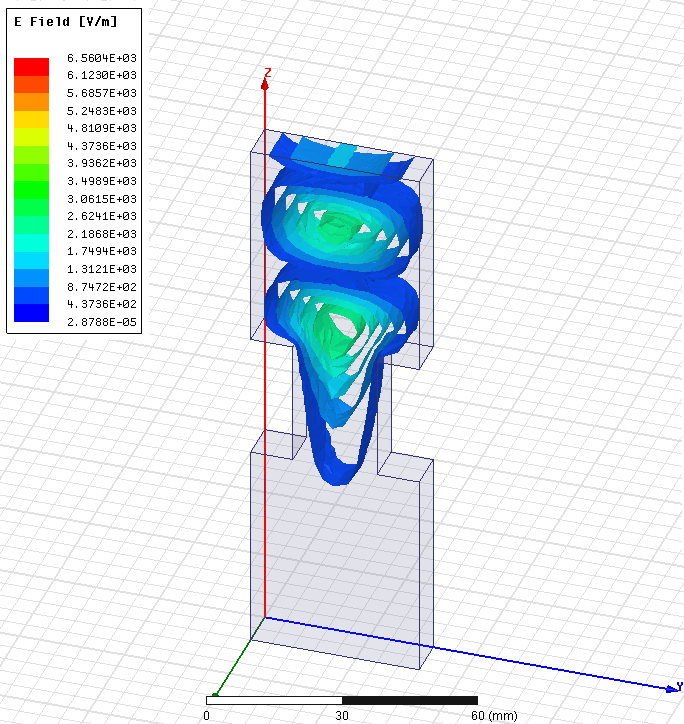
\includegraphics[width=\textwidth]{./mid_sec_20mm_wide_30mm_long/7ghz.png}
    \subcaption{The magnitude of the E-field at $f=\SI{7}{\giga\hertz}$.}
    \label{fig:2_2030_7ghz}
  \end{subfigure}\\
  \begin{subfigure}[b]{0.49\textwidth}
    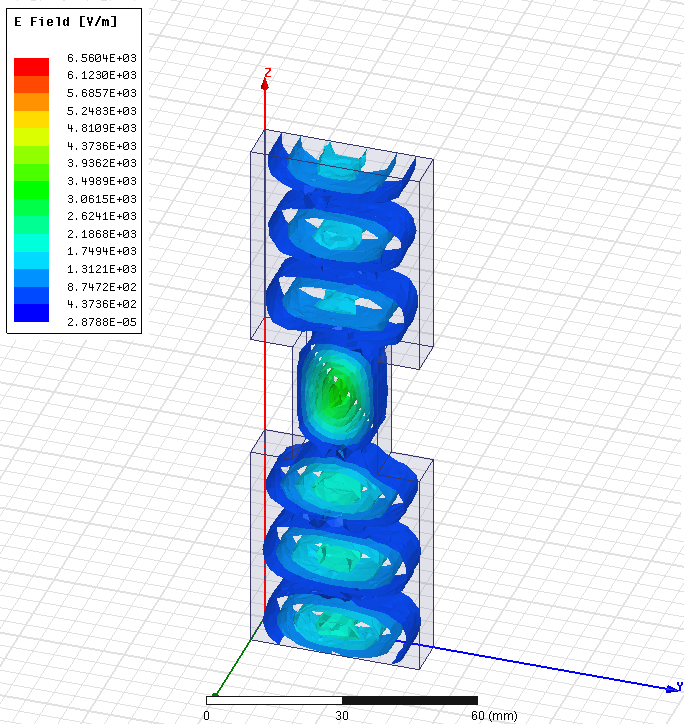
\includegraphics[width=\textwidth]{./mid_sec_20mm_wide_30mm_long/9ghz.png}
    \subcaption{The magnitude of the E-field at $f=\SI{9}{\giga\hertz}$.}
    \label{fig:2_2030_9ghz}
  \end{subfigure}
  \begin{subfigure}[b]{0.49\textwidth}
    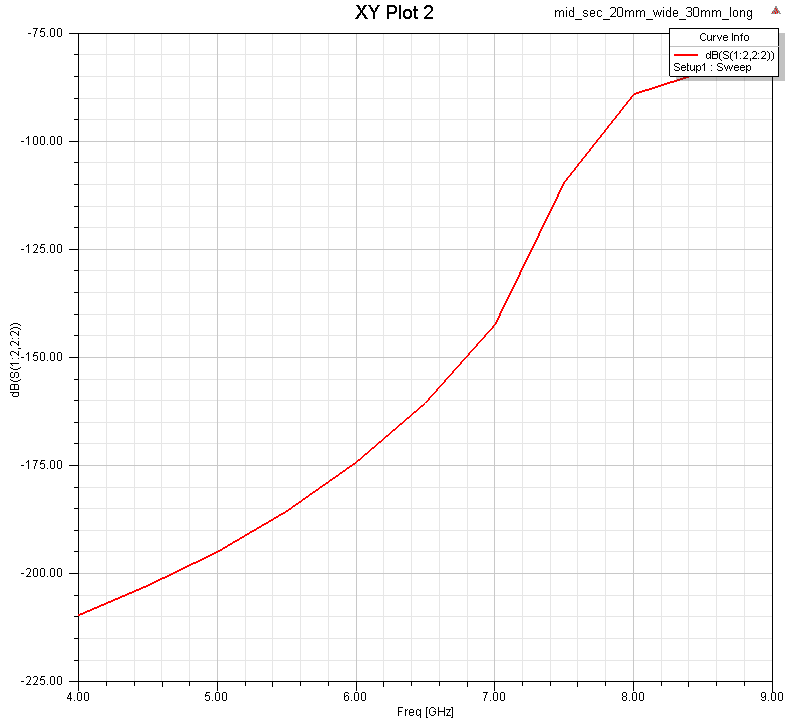
\includegraphics[width=\textwidth]{./mid_sec_20mm_wide_30mm_long/s1222.png}
    \subcaption{Output power of $TE_{20}$ ($S_{21}$).}
    \label{fig:2_2030_s1222}
  \end{subfigure}
  \caption{The figure shows the magnitude of the E-field and the $S_{21}$ parameter for a waveguide when the middle section's dimensions were $(x=\SI{10}{\milli\metre}, y=\SI{20}{\milli\metre}, z=\SI{30}{\milli\metre})$.}
  \label{fig:task2_2030}
\end{figure}

\subsection{Dimensions: y=20 mm, z=50 mm}
It can be seen in Figure~\ref{fig:task2_2050} that the cutoff frequency for this wave guide is above $\SI{9}{\giga\hertz}$ although the wave manages to propagate through the middle section.
\begin{figure}
  \centering
  \begin{subfigure}[b]{0.49\textwidth}
    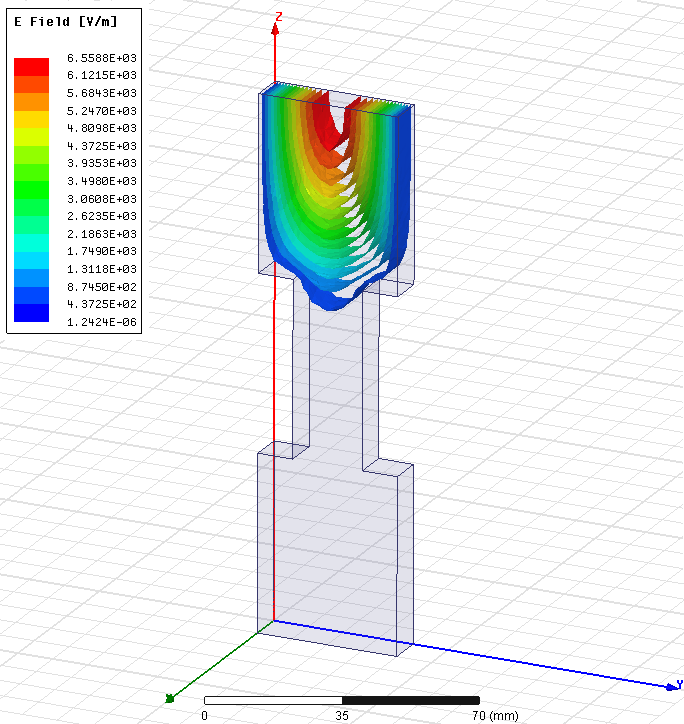
\includegraphics[width=\textwidth]{./mid_sec_20mm_wide_50mm_long/4ghz.png}
    \subcaption{The magnitude of the E-field at $f=\SI{4}{\giga\hertz}$.}
    \label{fig:2_2050_4ghz}
  \end{subfigure}
  \begin{subfigure}[b]{0.49\textwidth}
    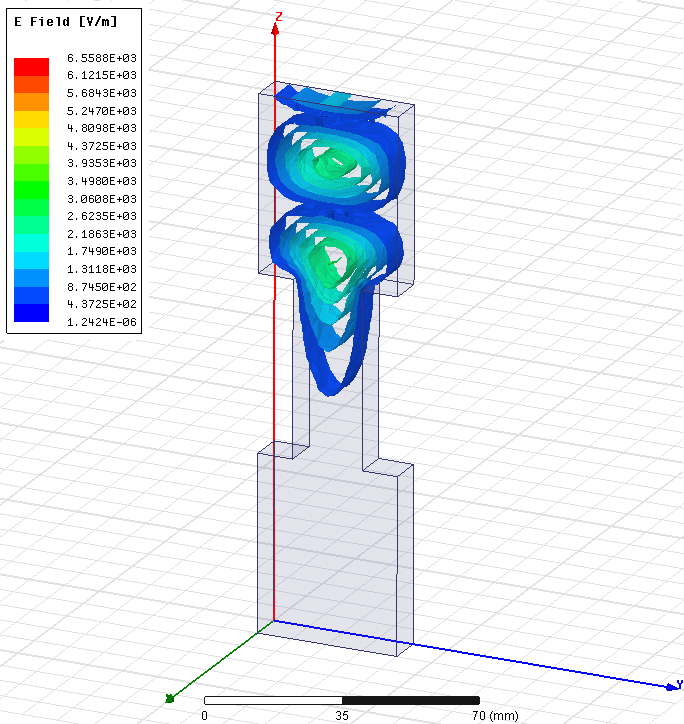
\includegraphics[width=\textwidth]{./mid_sec_20mm_wide_50mm_long/7ghz.png}
    \subcaption{The magnitude of the E-field at $f=\SI{7}{\giga\hertz}$.}
    \label{fig:2_2050_7ghz}
  \end{subfigure}\\
  \begin{subfigure}[b]{0.49\textwidth}
    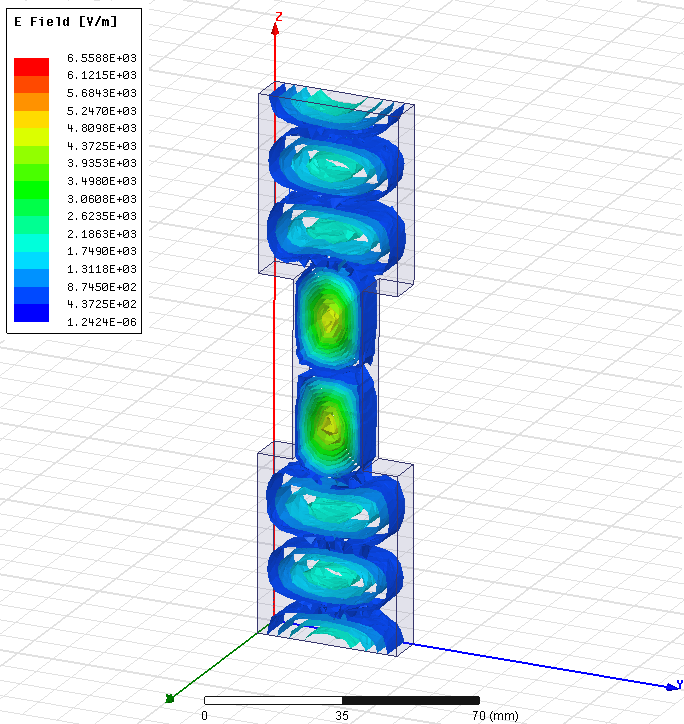
\includegraphics[width=\textwidth]{./mid_sec_20mm_wide_50mm_long/9ghz.png}
    \subcaption{The magnitude of the E-field at $f=\SI{9}{\giga\hertz}$.}
    \label{fig:2_2050_9ghz}
  \end{subfigure}
  \begin{subfigure}[b]{0.49\textwidth}
    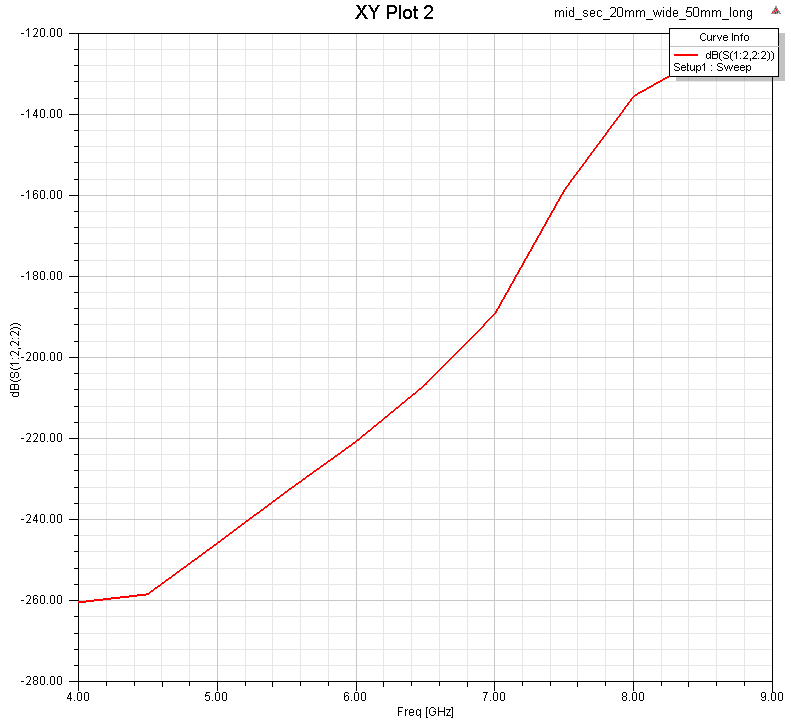
\includegraphics[width=\textwidth]{./mid_sec_20mm_wide_50mm_long/s1222.png}
    \subcaption{Output power of $TE_{20}$ ($S_{21}$).}
    \label{fig:2_2050_s1222}
  \end{subfigure}
  \caption{The figure shows the magnitude of the E-field and the $S_{21}$ parameter for a waveguide when the middle section's dimensions were $(x=\SI{10}{\milli\metre}, y=\SI{20}{\milli\metre}, z=\SI{50}{\milli\metre})$.}
  \label{fig:task2_2050}
\end{figure}

\end{document}